\section{Background Theory}
% \begin{itemize}
%     \item Husk rød tråd.
%     \item Vær generisk.
%     \item Bare inkluder konsept som blir relevante senere, eller som er brukt i nødvendige antagelser.
%     \item many of the concepts explained in this chapter were also explained in [TODO: fordypningsprosjekt].
%     \item The goal of this chapter is to explain all the concepts neccessary to understand how the trajeoctyr planning algorithm works.
%     Additionally, it should grant an understanding as to why the algorithm ended up the way it is.
% \end{itemize}
This chapter will introduce the concepts and theory neccessary to understand the design and intent behind the trajectoy planning algorithm, as well as the discussion on it's functionality.
The goal of the chapter is is to give the reader enough intuition of the applied theory that the proposed arguments and solutions should make sense. In addition, the chapter is structured
so that it should be easy to quickly navigate and read about specific topics.


\subsection{Vessel modelling } \label{CHAP: Vessel Modelling}
% --------- Genereal thoughts --------------------------
% Jeg tenker det er best å skrive om modellering i sammenheng med hvordan trajectory planning problemet blir satt opp i MATLAB med CasADi.
% \begin{itemize}
%     \item Kinematics \& Kinetics -\> Begge brukes i CasADi setup.
%     %\item Munk moment -> Potensielt relevant hvis jeg skriver om modellerings problemer
%     \item Her kan det også skrives om de spesifike tallverdiene som blir brukt i Masse, coriolis og dempnings -matrisene.
%     de er spesifike til Milliampere, funnet gjennom en rekke forsøk utfort av Anders Pedersen.
% \end{itemize}
% ---------- /General Thoughts--------------------------- 
% \begin{itemize}
%     \item A model in this context is just a way of describing how physical systems change over time.
%     \item There are many different ways to make models, and different models are suitable for modelling different aspects of the physical world.
%     \item The model described in this chapter, and used for the thesis, is a 3 \gls{DOF} nonlinear model based on the work of \cite{fossen2011handbook}.
%     \item The model can also incorporate wind and current disturbances, but they are omitted from this thesis.
%     \item The parameter values will vary from ship to ship, this thesis will operate with numbers for the NTNU milliampere ferry.
%     the parameters were found through testing by \cite{andersson2019casadi}
%     \item pose is parameterized in the \gls{NED} coordinate frame where the 
% \end{itemize}
% A mathematical model is a tool for describing physical systems and expressing how they change over time, models are not unique and there are many different ways of modelling a physical system, they all have strengths and weaknesses.
% % The model applied in this thesis is based on the theory and notation by \cite{fossen2011handbook},
A mathematical model is a tool for describing physical systems and expressing how they change over time, respond to external forces, and how stable the system might be. Models are very useful when designing control systems as
they translate the physical into equations that computers can understand. When making a model it is often useful to separate the dynamics of the different parts of the 
system we are interested in, these are the \gls{DOF} the system has, and is often the directions the system can move, though they can also just be
nondescript generalized coordinates. Deciding which \gls{DOF} to separate out and model the dynamics of is often what separates models from each other, it is pointless to model
an aspect of a system that there is no intent to interact with. For example a ship has six \gls{DOF}, see Figure \ref{FIG: Ship DOF}, for modelling a control system for stationkeeping
all six are important because stationkeeping involves keeping the whole ship as steady as possible. When modelling for path following on the other hand it is not
important what the heave, roll, or pitch of our vessel is and so the dynamics of those \gls{DOF} can safely be ignored. 
The model used to describe our vessel in this thesis is based on the theory and notation by (\cite{fossen2011handbook}), and is a 3\gls{DOF} nonlinear mass-damper system with
thruster dynamics and no external disturbances such as wind or currents. The dynamics of the vessel can be described by the differential equations below:

\begin{equation} \label{EQ: eta_dot}
    \bm{\dot{\eta}} = \textbf{R}(\psi)\bm{\nu}    
\end{equation}
\begin{equation} \label{EQ: Vessel Dynamics}
    \textbf{M}\bm{\dot{\nu}} + \textbf{C}(\bm{\nu})\bm{\nu} + \textbf{D}(\bm{\nu})\bm{\nu} = \bm{\tau}
\end{equation} %(TODO linjen som følger equation er SAMME SETNING.)
% where $\bm{\eta}$ is the pose of the vessel, parameterized in the tangental plane \gls{NED} where the x-axis 
%points towards true north, the y-axis east and the z-axis down towards the center of the planet.
% The \gls{NED} frame can be said to be inertial for short distance control objectives.
% Here, the vector $\bm{\eta}$ is a column vector with the vessel's North, East and Heading values, 
% which are the three \gls{DOF} of the system. The $\bm{\nu}$ vector is a column vector containing
% the vessel's velocities parameterized in the BODY frame, namely surge, sway, and yaw rate. 
% In the BODY frame there are no fixed rules for where the axis are pointing, but the common convention for modelling
% vehicles is that the x-axis points along the lognitudal axis of the vessel, the y-axis points along the lateral axis
% and the z-axis points along the vertical axis. This is also seen in Figure \ref{FIG: Ship DOF}.
% The anchor point for the BODY frame is arbitrary but always fixed to the vessel and moves with it. 
% \textbf{R} is a rotational matrix about the heading ($\psi$) of the vessel and it transform the BODY velocities into
% NED movement. 
% The Rotation matrix, as well as pose, velocity, and the thruster vector $\bm{\tau}$ are:
where $\bm{\eta}$ is the pose of the vessel parameterized in the tangetnal plane \gls{NED}, $\bm{\nu}$ are
the velocities of the vessel, parameterized in the BODY frame of the vessel. And $\bm{\tau}$ are forces and torque applied to the
system. The \gls{NED} frame can be said to be inertial for short distance control objectives, and in this frame 
the x-axis points towards true north, the y-axis points east and the z-axis points down towards the center of the planet.
Thus; $\bm{\eta} = [x\ , \ y \ , \ \psi]^T \in \mathbb{R}^{3}$ are the vessel's North, East and Heading values, 
which are the three \gls{DOF} of the system. The velocities $\bm{\nu} = [u\ , \ v \ , \ r]^T \in \mathbb{R}^{3}$ are the
surge, sway, and yaw rate of the vessel. In the BODY frame there are no fixed rules for where the axis are pointing, but the common convention for modelling
vehicles is that the x-axis points along the lognitudal axis of the vessel, the y-axis points along the lateral axis
and the z-axis points along the vertical axis. This is also seen in Figure \ref{FIG: Ship DOF}.
The anchor point for the BODY frame is arbitrary but always fixed to the vessel and moves with it. 
The forces and toruqe $\bm{\tau} = [F_{X}\ , \ F_{Y} \ , \ F_{N}]^T \in \mathbb{R}^{3}$ are the forces acting along
the logitudal axis, lateral axis, and torque about the vertical axis of the vessel's BODY frame. The rotation matrix \textbf{R}($\psi$) rotates the BODY velocities into \gls{NED} movement about the
vessel's heading, and is definied as:
\begin{equation}
    \textbf{R}(\psi) = \begin{bmatrix}
                        cos\psi &   -sin\psi & 0\\
                        sin\psi & cos\psi    & 0\\
                        0       &   0        & 1
                        \end{bmatrix}
\end{equation}


\begin{figure}[ht]
    \centering
    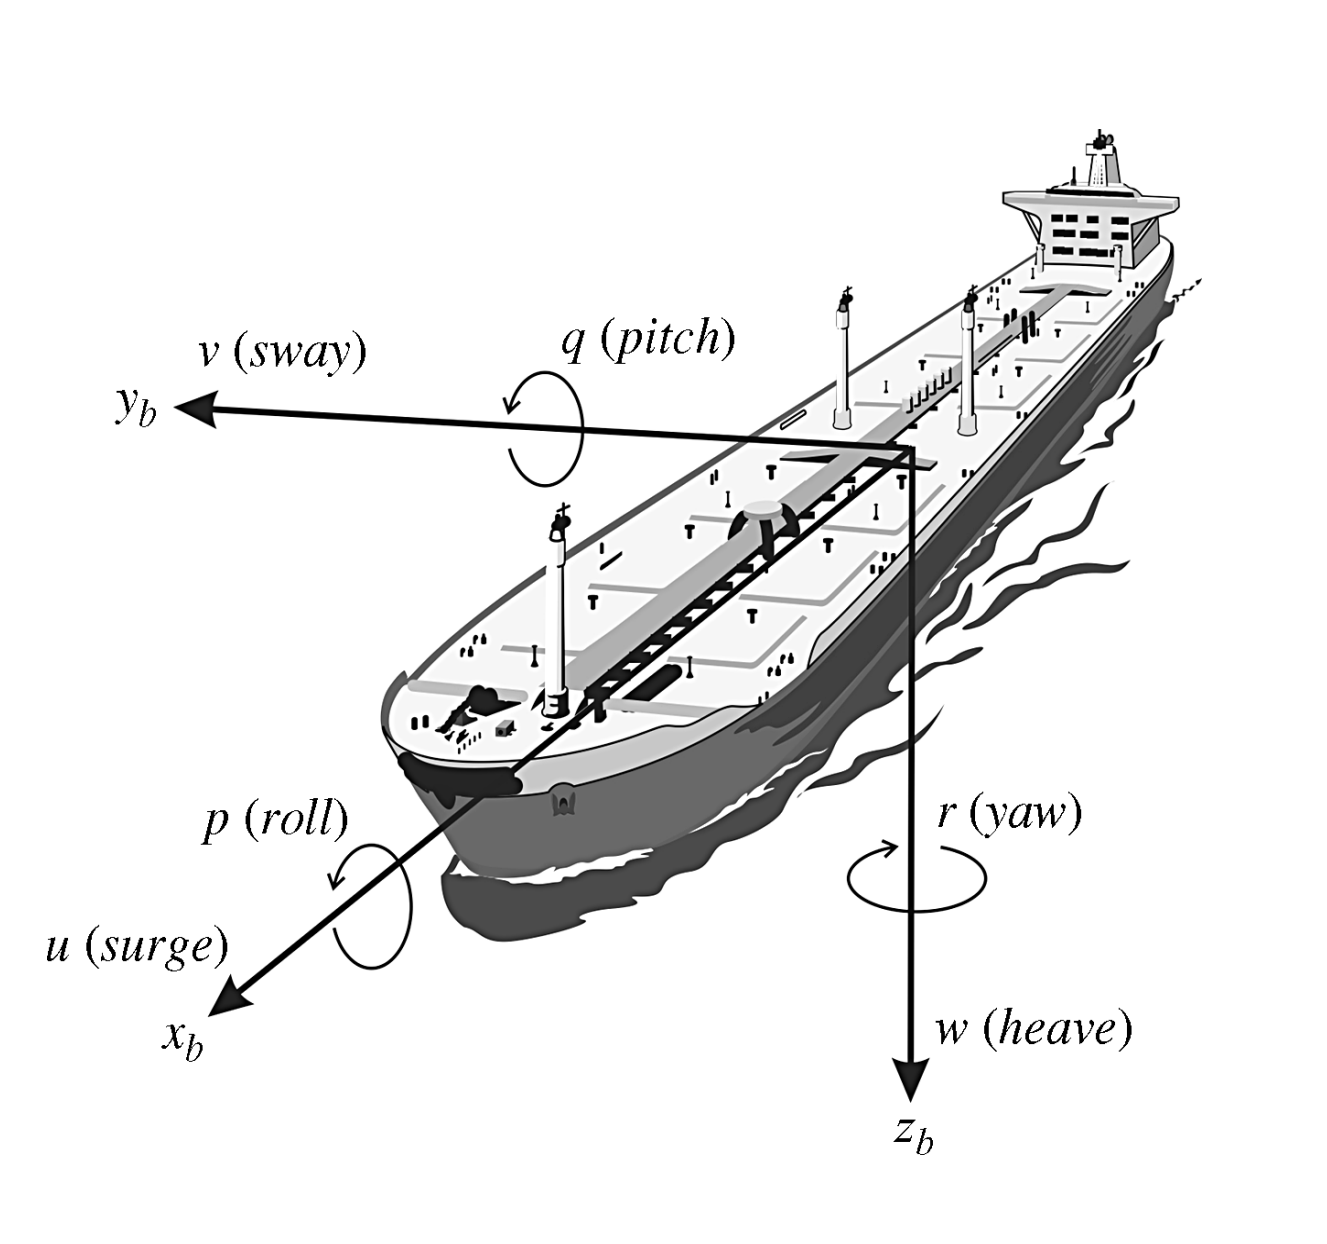
\includegraphics[height=0.35\textheight]{Images/SHIPDOF_FOSSEN.png}
    \caption{A ships 6 degrees of Freedom, from (\cite{fossen2011handbook}).} %(TODO: TA BEVIST VALG, PUNKTUM ELLER IKKE.)
    \label{FIG: Ship DOF}
\end{figure}


% \begin{equation} % TODO: FLYTT INN I FLYTTEKST
%     \bm{\eta} = \begin{bmatrix}
%                 x   &    y  &    \psi
%                 \end{bmatrix}^T
% \end{equation}
% \begin{equation} % TODO: FLYTT INN I FLYTTEKST
%     \bm{\nu} = \begin{bmatrix}
%                  u   &   v  &    r
%                 \end{bmatrix}^T
% \end{equation} % TODO: FLYTT INN I FLYTTEKST
% \begin{equation} \label{EQ: Tau}
%     \bm{\tau} = \begin{bmatrix}
%                 F_{X}   &   F_{Y}  &   F_{N}
%                 \end{bmatrix}^T
% \end{equation}

% \begin{itemize}
%     \item $\eta$ is defined in the \gls{NED} reference frame, $\nu$ is defined in BODY frame, briefly explain what that means.
%     \item The M and C matrices are a combination of Rigid body and hydrodynamic added mass matrices
%     \item Fully computing the M and C matrices is a lot of work, for milliampere the work has already been conducted
%     by Andreas Pedersen.
%     \item If the model values are to be found through experiementation it's senseless to separate Rigid body and hydrodynamic added mass.
%     The matrices then become:
% \end{itemize}

In \eqref{EQ: Vessel Dynamics} the \textbf{M} matrix is the inertia matrix of the system, which describes how 'heavy' the \gls{DOF} are to nudge, in
addition to the vessel's inherent inertia from being massive the vessel must also push water out of the way when it moves, this is what is known as
hydrodynamic added mass and is linearly added to the inertia matrix. The coriolis matrix \textbf{C} also has to include hydrodynamic added mass,
however for the purpose of this thesis it is not important to know the parameters for either of these matrices or for the dampening matrix \textbf{D}.
That is because a trajectory planning algorithm needs to work regardless of vessel parameters, (\cite{pedersen2019optimization}) explains more in-depth
how system parameters can be found. Continuing on, the dampening matrix is a linear combination of the linear dampening stemming from water
viscosity and non-linear dampening from cross-flow, once again the parameters themselves are not strictly relevant to this thesis, but intuition is
important. The result are matrices in the following form:

\begin{equation} \label{EQ: Mass}
    \textbf{M} = \begin{bmatrix}
                m11 &   m12 &   m13\\
                m12 &   m22 &   m23\\
                m31 &   m32 &   m33
                 \end{bmatrix}
\end{equation}

\begin{equation} \label{EQ: Coriolis}
    \textbf{C}(\bm{\nu}) =  \begin{bmatrix}
        0             &     0       &   c13(\bm{\nu})\\
        0             &     0       &   c23(\bm{\nu})\\
        c31(\bm{\nu}) &c32(\bm{\nu})&   0
                            \end{bmatrix}    
\end{equation}

\begin{equation} \label{EQ: Dampening}
    \textbf{D}(\bm{\nu}) =  \begin{bmatrix}
        d11(\bm{\nu}) &     0       &   0\\
        0             &d22(\bm{\nu})&d23(\bm{\nu})\\
        0             &d32(\bm{\nu})&d33(\bm{\nu})
                            \end{bmatrix}       
\end{equation}

The dampening matrix can be a bit of a compuational nightmare and can be simplified to a linear and diagonal matrix without too much
of a detrimental impact on our simulations. The justification for this simplification is the underlying assumption that the reference output
from the trajectory planner algorithm will be parsed through a final control module that will account for dampening. The risk is that
the end result from the trajectory planner turns out to be infeasible, but that's a problem for another thesis.

\begin{equation} \label{EQ: Dampening_Simple}
    \textbf{D}(\bm{\nu}) = \begin{bmatrix}
                            d11 &   0   &   0\\
                            0   &   d22 &   0\\
                            0   &   0   &   d33
                            \end{bmatrix}
\end{equation}

Finally, a word on heading vs course. Throughout this thesis the terms course and heading might be used interchangeably, but the words are strictly not synonymous.
Heading is equivalent with yaw as both denote a rotation about the vessel's third axis, the difference between the two is that yaw is often a relative term describing
a change by some degrees from one arbitrary pose to another. Heading is an absolute term and is often based on compass directions, meaning 0\textdegree heading
equates to the nose of the vessel pointing towards true north. Neither heading nor yaw is equivalent with course, which is strictly the direction
of travel relative to true north. In a simplified world void of disturbances heading and course will align during straight line
travel, but external forces such as wind or currents will cause the two angles to deviate. Likevise sideslip caused by a non-zero sway velocity when turning will 
also introduce a deviation between course and heading (\cite{fossen2011handbook}). However this difference is mostly unrelated to the work put forth in this thesis, 
and so the terms heading and course might be used interchangeably. Althought it often makes sense to deliberately pick one
term over the other.


\subsection{Trajectory Planning} \label{CHAP: Trajectory planning}
(TODO: Savner et lite avsnit om Shortest Signed Angle eller WrapTo2Pi.)
% --------- Genereal thoughts --------------------------
% \begin{itemize}
%     \item How to get from A to B.
%     \item Multiple methods, all with pros and cons, skriv liten oversikt.
%     \subitem LOS, OCP, Machine Learning, osv.
%     \subitem Kanskje ikke så veldig viktig å snakke om andre metoder enn OCP.  
%     \item Important factors to consider:
%     \subitem Time horizon / length of planning period.
%     \subitem Trajectory safety with respect to ship capabilities.
%     \subitem \gls{COLREGs} compliance 
%     with respect to expected behaviour.
%     \subitem osv.
%     \item Litt dypere inn i numerisk optimalisering og MPC, og LOS ettersom det kommer til å bli brukt igjen senere.
%     \item Disambiguate Path vs Trajectory
%    % \item Først oversikt, deretter enten nytt kapittel eller delkapittel om 
%    % den spesifikke metoden jeg skal bruke, forklar numerisk optimalisering, MPC, LOS guidance, hvordan alt kombineres til å bli min algoritme, in theory.
% \end{itemize}
% --------- /Genereal thoughts --------------------------
% \begin{itemize}
%     \item Core concept. Path VS Trajectory.
%     \item Many ways of doing it.
%     \item chosen method for this thesis.
%     \item Numerical optimization, OCP, NLP, MPC.
% \end{itemize}
% Because the model for describing the dynamics of our vessel is a set of ordinary differential equations we can solve them for the input we need
% to achieve any desired state. And because the dynamics are time-invariant we can solve for any future time interval given initial conditions.
Because the vessel dynamics are described by a model expressed as a set of time-invariant ordinary differential equations, any desired state
can be reached by solving for the sequence of inputs that will take the vessel from a given initial condition to said state. In the context of this
thesis "state" refers to the pose, $\bm{\eta}$, of the vessel. The simplest application of this would be moving in a straight line from point A to point B.
The solution is simply to find the input sequence which turns the vessel to the correct course and then maintaining a forward speed until point B is reached.
The straight vector line from point A to point B can be thought of as the desired or reference path, while the sequence of states achieved by applying the 
input sequence is the trajectory. Instead of having just one destination there might be multiple waypoints forming the path, and the optimal
input sequence that makes the controlled vessel, from here on called "Own Ship" (OS), travel along the path depends on what criteria are considered important. A trajectory generated with fuel
economy in mind might look very different from a trajectory generated with shortest transit time in mind, even if both are following the same path.
Other factors such as obstacles or disturbances will also influence the trajectory, combining all the factors and generating the desired
input sequence is the act of trajectory planning.

There are many methods for trajectory planning. Some are conceptually simple and fast to compute, but lack robustness and situational adaptability.
Other method can be incredibly complex and and computationally expensive, but in return incredibly robust to disturbances and adaptable to
any situation. An example of a simple trajectory planner would be a \gls{LOS} guidance law while something extremely advanced would be training a machine
learing algorithm. For an overview: in this thesis a \gls{LOS} guidance law will be applied to generate a reference trajectory, the reference is then used as part of a
formulation of an \gls{OCP} with a cost to penalize deviation from the reference in addition to other factors.
The \gls{OCP} is then discretized as a \gls{NLP} problem using a method called direct multiple shooting,
finally the \gls{NLP} is solved with an \gls{IPOPT} solver.
One of the big advantages of \gls{OCP} is that it allows formulating constraints directly on the states, 
which is a big deal when it comes to collosion avoidance.

\subsubsection*{Line of Sight Guidance} \label{CHAP: LOS GUIDANCE} % TODO: FÅ INN FIGUR.
% \begin{itemize}
%     \item Path following algorithm.
%     \item Cross track and along track errors.
%     \item integral action.
%     \item course control will not be neccessary.
%     \item Only considering the horizontal control.
%     \item Suppressing cross track error towards zero gives the desirec course to follow.
%     \item When the along track error is below a certain threshold k = k + 1 (move to the next waypoint)
%     \item \cite{lekkas2013line}
% \end{itemize}

This guidance method is perhaps the most intuitive; consider the waypoints WP\textsubscript{k} and WP\textsubscript{k+1}, the simplest path
from one to the other would be straight line. Therefor the most obvious control method would be to maneuver onto the straight line, and
follow it along to the end. The distance of the \gls{OS} to the straight line is called the cross track error $y_e$ and the distance along the line
to the end is called the along track error $x_e$. The along track error is not of any importance to this thesis, it is assumed that the controlled
vessel will maintain a steady velocity, and there are no temporal constraints on reaching the goal.

As explained in (\cite{lekkas2013line}); given the \gls{OS}'s position (x,y), the cross track and along track errors from the straigth line as defined by WP\textsubscript{k} (x\textsubscript{k},y\textsubscript{k})
and WP\textsubscript{k+1} (x\textsubscript{k+1}, y\textsubscript{k+1}) are:
\begin{equation}\label{EQ: cross and along track error} %% Along track and Cross Track error
    \begin{bmatrix}
        x_e \\
         ye
    \end{bmatrix} = \textbf{R}^T(\gamma_p) \begin{bmatrix}
                                            x - x_k \\
                                            y - y_k
                                            \end{bmatrix}
\end{equation}
where R is the rotation matrix from the inetiral frame to the straight line's frame. Here, $\gamma_p$ is the horizontal path-tangental angle,
or the 'angle' of the straight line path in relation to the inetrial frame if that makes more sense, see Figure \ref{FIG: LOS_decomp} for a visual
decomposition. The rotation matrix \textbf{R} is given by:
\begin{equation} %% Rotation matrix R(gamma)
    \textbf{R}(\gamma_p) = \begin{bmatrix}
                            cos(\gamma_p) & -sin(\gamma_p) \\
                            sin(\gamma_p) & cos(\gamma_p)
                            \end{bmatrix}
\end{equation}
with $\gamma_p$:
\begin{equation} %% Calculating Gamma
    \gamma_p = \textrm{atan2}(y_{k+1} - y_k , x_{k+1} - x_k)
\end{equation}
The control objective is to drive $y_{e}(t) \rightarrow 0.$ as t trends towards infinity. Assuming a steady velocity this is done by
selecting a course that steers the \gls{OS} in the direction that reduces $y_e$. How fast the error $y_e$ is suppressed is
tuned by a proportional gain factor, $\varDelta$, that is often called look ahead distance. The desired heading is given by:
\begin{equation} %% Calculating psi_d
    \psi_d = \gamma_p + \arctan(\frac{-y_e}{\varDelta})
\end{equation}
and consequently desired course:
\begin{equation}
    \chi_d = \psi_d + \beta
\end{equation}
where $\beta$ is the sideslip of the \gls{OS}. Because real life situations are rarely, if ever, devoid of disturbances that introduce
sideslip and crab angles there is one common improvement that can be made: Integrate the cross track error and use both current cross track error
and it's integral when calculating desired heading. The equation for $\dot{y}_{int}$ and $\psi_d$ then become:
\begin{equation}
    \dot{y}_{int} = y_e
\end{equation}
\begin{equation}
    \psi_d = \gamma_p - \arctan(K_{p}y_e + K_{i} y_{int})
\end{equation}
where K\textsubscript{p} and K\textsubscript{i} are gain parameters proportional to the lookahead distance, typically $K_p = (1/\varDelta)$, $K_i = Kp*\kappa$
with $\kappa > 0$ being some design variable.

\begin{figure}
    \centering
    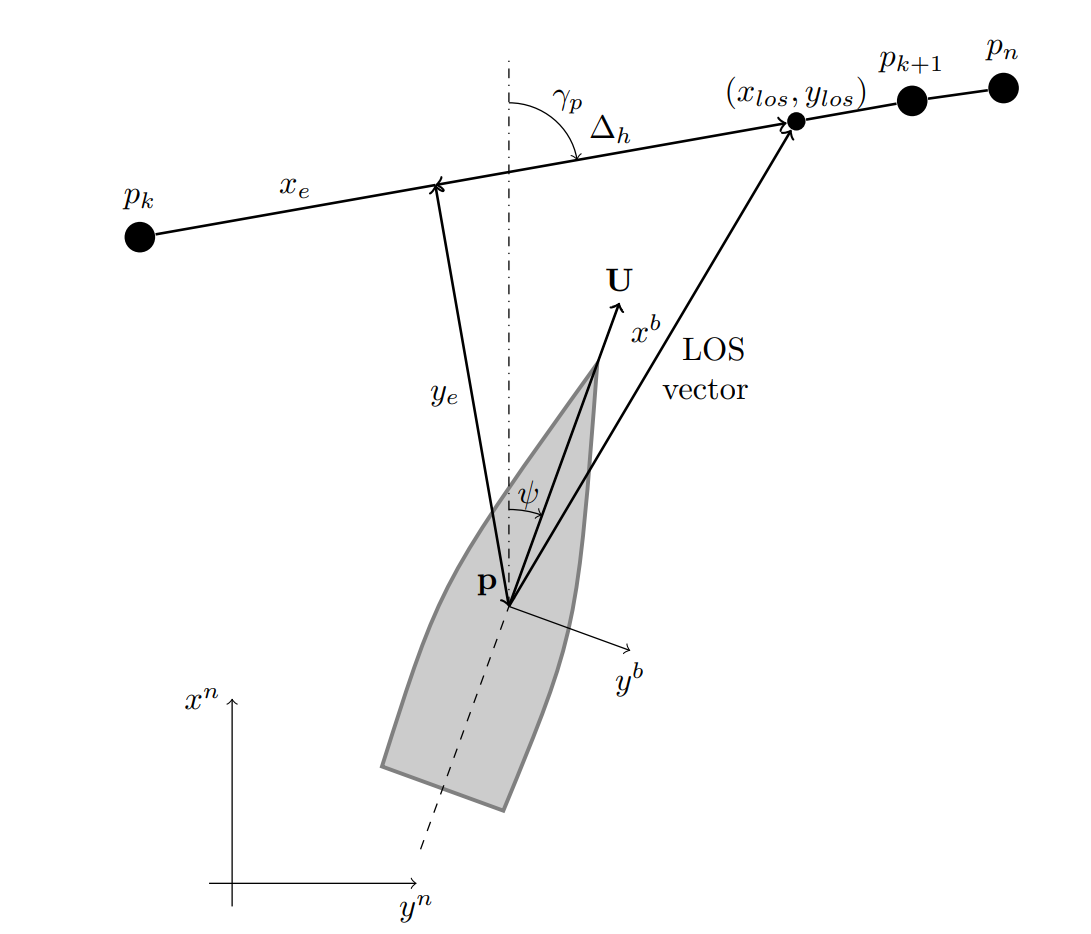
\includegraphics[width = 0.7\textwidth]{Images/LOS_decomp.png}
    \caption{Line of sight guidance geometry for straight lines, here with zero sideslip. Image courtesy of (\cite{lekkas2013line})} % TODO: Used without permission?
    \label{FIG: LOS_decomp}
\end{figure}

A reference trajectory is generated by using the LOS law as described to guide the contolled vessel from it's initial position through all the waypoints, and
saving the desired positions and velocities after each time step. For a path with more than two waypoints a simple index incrementation can be used when the
vessel is within a certain distance from it's current target waypoint. The reference trajectory from $t_0$ to N (TODO: Dette er vel teknisk sett blanding av diskret og kontinuerlig notasjon) iterations of \gls{LOS} applications is of the form:
\begin{subequations}
    \begin{align}
        \overline{\bm{\eta}}_{ref} \quad & = [\bm{\eta}_{t0} \ , \ \bm{\eta}_{t+1} \ , \ \dots \ , \bm{\eta}_N] \in \mathbb{R}^{3 \times N} \\ 
        \overline{\bm{\nu}}_{ref} \quad & = [\bm{\nu}_{t0} \ , \ \bm{\nu}_{t+1} \ , \ \dots \ , \bm{\nu}_N] \in \mathbb{R}^{3 \times N}
    \end{align}
\end{subequations}

\subsubsection*{Optimal Control Problem} \label{CHAP: OCP}
% \begin{itemize}
%     \item Equations.
%     \item Model Predictive Control is simulating the dynamics of the system with a desired control objective and then applying the first states as
%     reference for the vessel's control system. After actuation new measurements are taken and the model is simulated again from the new initial conditions.
%     \item Many ways to solve an optimization problem, often quite difficult due to Continuous dynamics.
%     \item cite \cite{breivik2017mpc} for a quick look and equation formulation.
%     \item cite \cite{wright1999numerical} For a comprehensive lesson on optimal control.
% \end{itemize}
Numerical optimization is a vast field within mathematics, (\cite{wright1999numerical}) explains it well: There are no universal optimization algorithm. Instead an algorithm must be tailored to the optimization
problem. Within the context of trajectory planning there are different parameters to optimize for, some examples are: maintaining steady velocity, suppressing sway, minimalizing
fuel waste, minimizing distance to goal, and there are many more. The general expression for an optimization problem can be written as simple as:
\begin{subequations}
    \begin{align}
    \underset{x\in \textbf{R}^n}{\textrm{Minimize}} \quad & f(x) \\
        \textrm{Subject to:} \quad & c_i(x) = 0, \quad i \in \mathcal{E} \\
                             \quad & c_i(x) \geq 0, \quad i \in \mathcal{I} 
    \end{align}
\end{subequations}
% \begin{itemize}
%     \item However a better generalized formulation was made in \cite{breivik2017mpc}, it's basically the same but expressed in a way that will be easier to use later.
%     \item The cost function is 
% \end{itemize}
Where $f(x)$
is the objective function where the optimization objectives are encoded.
The functions $c_i$ are constraint on the system which $f(x)$ exists in, and $\mathcal{E}$ and $\mathcal{I}$ are indices
pertaining to if the constraint $c_i$ is an equality or inequality constraint. In the context of this thesis the thing to minimize is some nebulous cost function
associated with path following, and the constraints are the physical model of the system that guarantees feasibility as well as safety constraints to avoid collisions.
The cost function is then some function of the vessel's state, reference trajectory, and control input. The two constraints are the system dynamics from \eqref{EQ: Vessel Dynamics}
and \eqref{EQ: eta_dot}. And then additional constraints for collision safety and initial conditions. A new general \gls{OCP} definition is thus given by the following:

\begin{subequations}
    \label{EQ :OCP description}
\begin{align}
    % \textrm{Minimize} \quad & \textbf{F}(\boldsymbol{\eta}(t), \textbf{u}(t)) \label{eq:OCP-a} \\ 
    % \textrm{subject to} \quad & \dot{\boldsymbol{\eta}}(t) = \textbf{L}(\boldsymbol{\eta}(t), \textbf{u}(t)) \label{eq:OCP-b} \\
    % \quad & \textbf{h}(\boldsymbol{\eta}(t), \textbf{u}(t)) \leq \textbf{0} \label{eq:OCP-c}\\
    % \quad & \boldsymbol{\eta}(t_0) = \boldsymbol{\eta}_0 \label{eq:OCP-d}
    \textrm{Minimize} \quad & {L}(\bm{\theta}(t), \bm{\theta}_{ref}(t), \bm{\tau}(t)) \\
    \textrm{Subject to:} \quad & \dot{\bm{\theta}}(t) = \textbf{J}(\bm{\theta}, \bm{\tau}) \\
                         \quad & \textbf{h}(\bm{\theta}(t), \bm{\tau}(t)) \leq \bm{0} \\
                         \quad & \bm{\theta}(t_0) - \overline{\bm{\theta}}_0 = \bm{0}
\end{align}
\end{subequations}
where L is the cost function, $\bm{\theta} = [\bm{\eta}^T \ , \ \bm{\nu}^T]^T$ and $\bm{\tau}$ is still the same as in \eqref{EQ: Vessel Dynamics}. 
\textbf{J}($\bm{\theta}, \bm{\tau}$) Are the model dynamics \eqref{EQ: eta_dot}, \eqref{EQ: Vessel Dynamics}. $\overline{\bm{\theta}}_0$ are the
given intial conditions of the system.
The solution to the optimization problem is the series of inputs $\bm{\tau}$ which minimizes the integral of the cost L 
from t\textsubscript{0} to t\textsubscript{end}. And L has the form of a quadratic function
akin to a weighted least squares: (TODO: Eh, grei formulering?)
\begin{equation}
    L(\bm{\theta}(t), \bm{\theta}_{ref}(t), \bm{\tau}(t)) = (\bm{\theta}(t) - \bm{\theta}_{ref}(t))^T \textbf{Q} (\bm{\theta}(t) - \bm{\theta}_{ref}(t)) + \textbf{K}_\tau \bm{\tau}^2
\end{equation}
Where the diagonal of the \textbf{Q} matrix are the weight coefficients of deviating from the reference
and \textbf{K}\textsubscript{$\tau$} is another weighting matrix for applied forces and torques.

Solving the \gls{OCP} can be done using a multitude of methods, \cite{breivik2017mpc} suggest discretizing 
the \gls{OCP} into a \gls{NLP} using a method called direct multiple shooting.


\subsubsection*{NonLinear Programming} \label{CHAP: NLP}
% \begin{itemize}
%     \item discretized formulation of the OCP, using among many methods, Direct Multiple shooting.
%     \item I don't really understand this stuff too much.
%     \item Direct Multiple Shooting explanation needed.
%     \item shooting gaps.
%     \item cite \cite{gros2017Lecture} for direct multiple shooting
%     \item cite \cite{andersson2019casadi} Casadi for constructing the NLP in a 
%     computer friendly way, and \cite{wachter2006implementation} for IPOPT
% \end{itemize}
% \begin{itemize}
%     \item Direct multiple shooting is a discretized formulation of the \gls{OCP} where both the states and the control
%     inputs are explicitly defined as decision variables.
%     \item Because direct multiple shooting means the selected solver is 'free' to place the states and inputs wherever it wants
%     we must employ shooting constraints to enforce a physically feasible trajectory. This is called closing the shooting gaps.
%     \item A solver is an algorithm decined to crunch the NLP problem, 
%     in this thesis we will use an \gls{IPOPT} solver \cite{wachter2006implementation}.
%     \item To help formulate the \gls{NLP} a framework provided by \cite{andersson2019casadi} will be used.
%     \item The shooting gaps constraints are created by integrating forward one time step at each control interval
%     with a RK4 mehtod, which gives us a discret value $\omega$\textsubscript{k+1} using the continuous function $\textbf{f}(\bm{\omega})$. 
%     For each control interval k there must be a shooting gap constraint $\textbf{F}(\bm{\omega}_k) - \bm{\omega}_{k+1} = 0$. 
%     These shooting gap constraints are placed in \textbf{g}($\bm{\omega}$)
%     \item To avoid collisions constraints pertaining to illegal positions are also placed in \textbf{g}($\bm{\omega}$)
%     \item To make sure decision variables that are outside of 'legal' limits aren't searched for; The decision variables $\bm{\omega}$ are constrained by
%     upper and lower bounds which limits the search space with an upper and lower bound. 
%     This doesn't matter much for decision variables that are states, but matters a lot for velocities. ???
% \end{itemize}
The author would like to note that the technique used in this section, direct multiple shooting, is outside the scope of the author's knowledge.
Everything the author knows about this technique was learned over the course of the master thesis project, and it's highly recommended to read the full formulation by (\cite{breivik2017mpc})
which is the formulation that the implementation for this thesis heavily builds upon. Another great resource for direct multiple shooting are the video lectures of (\cite{gros2017Lecture}).
Also note that functions and definitions from the previous section on \gls{OCP} carry over, for example $\bm{\theta} = [\bm{\eta}^T \ , \ \bm{\nu}^T]^T$ still holds.\newline
Direct multiple shooting is a \gls{OCP} discretization technique where both the states and control inputs are excplicitly defined as decision variables.
The \gls{NLP} is then a reformulation of \eqref{EQ :OCP description} where L is redefined as a discretized cost function with $N_p$ control intervals steps:
\begin{equation} %(TODO: GÅ GJENNOM DETTE)
    \Phi(\bm{\omega}, \bm{\omega}_{ref_{1:N_p}}) = 
    \sum_{k=0}^{N_{p}-1} ((\bm{\theta}_{k+1} - \bm{\theta}_{ref_{k+1}})^T Q (\bm{\theta}_{k+1} - \bm{\theta}_{ref_{k+1}}) + K_{\bm{\tau}} \bm{\tau_k}^2)
\end{equation}
where $\bm{\omega} = [\bm{\theta}_0^T \ , \ \bm{\tau}_0^T \ , \ ... \ , \ \bm{\theta}_{N_{p}-1}^T \ , \ \bm{\tau}_{N_{p}-1}^T \ , \ \bm{\theta}_{N_{p}}^T]^T \in \mathbb{R}^{9N_{p}+6}$
% (TODO: Er det rett at det skal være $N_{p-1}$ i subscript og ikke $NP-1$?).
is a vector containing $9N_p + 6$ decision variables. % and $\bm{\theta}$ is the same as it was in \ref{EQ :OCP description}.
Because $\bm{\tau}_k$ is the control input; it is separated out as it's own part of the function. % Because $\bm{\tau}_k$ does not have an accociated reference in this thesis; it is separated out as it's own part of the function.
Here, \textbf{Q} is still a sparse 6x6 matrix where the diagonal contain the tuning parameters,
and \textbf{K}\textsubscript{$\bm{\tau}$} are still tuning parameters on control input. The complete NLP will end up in the form of:
\begin{subequations}
    \label{EQ:NLP}
    \begin{align}
        % \min_{\boldsymbol{\omega}} \quad & \textbf{L}(\boldsymbol{\omega}) \label{eq:NLP-1} \\
        % \textrm{subject to} \quad & \boldsymbol{\omega}_{lb} \leq \boldsymbol{\omega} \leq \boldsymbol{\omega}_{ub} \\ 
        % \quad & \textbf{g}_{lb} \leq \textbf{g} \leq \textbf{g}_{ub}
        \min_{\bm{\omega}} \quad & \bm{\Phi}(\bm{\omega}, \bm{\omega}_{ref_{1:N_p}}) \\ %% (TODO: er det rett å ha min_w?)
        \textrm{Subject to:} \quad & \bm{\omega}_{lb} \leq \bm{\omega} \leq \bm{\omega}_{ub} \\
                            \quad & \textbf{g}(\bm{\omega})_{lb} \leq \textbf{g}(\bm{\omega}) \leq \textbf{g}(\bm{\omega})_{ub}
    \end{align}
\end{subequations}
where $\bm{\omega}_{lb}$ and $\bm{\omega}_{ub}$ are the lower and upper bounds on the permitted values for $\bm{\omega}$, this is meant to limit the decision variables to 
physically feasible values when solving the NLP. \textbf{g}($\bm{\omega}$) is a vector of constraint functions that are similarly bound
by an lower and upper bounds, where the bounds define if the function in \textbf{g} is an equality or inequality constraint. Due to the way direct multiple shooting
defines the decision variables the programmed solver that solves the \gls{NLP} is free to place the states and velocities anywhere within the constraints. It is therefor
important to implement equality constraints that force the ending of one control interval and the beginning of the next to line up. This is called closing the shooting gaps, 
an illustration of what shooting gaps are can be seen in Figure \ref{FIG: Shooting Gaps}. These equality constraints are called shooting constraints and to create them begin
by defining an integrator function $\textbf{F}(\bm{\theta}_{k}, \bm{\tau}_k)$ using any technique, in this thesis the following \gls{RK4} method will be used:

\begin{figure}
    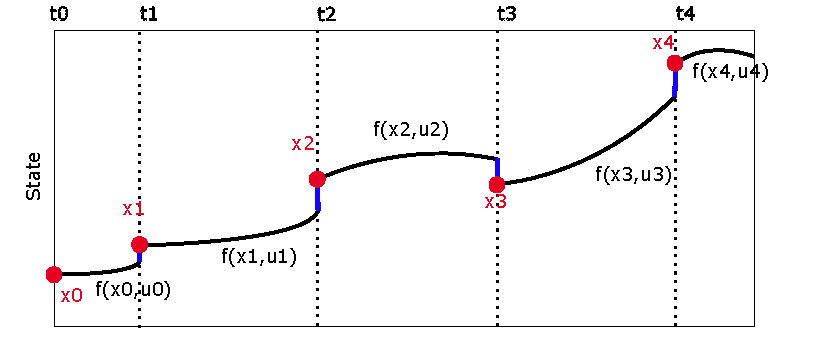
\includegraphics[width=\textwidth]{Images/MultipleShooting.pdf}
    \caption{A physically feasible trajectory is formed by "pinching" the shooting gaps close. Reproduction from (\cite{gros2017Lecture}).}
    \label{FIG: Shooting Gaps}
\end{figure}

\begin{equation}
    \label{EQ: RK4}
    \begin{split}
    k_1 = \quad & \textbf{f}(\bm{\theta}_{k} \ , \ \bm{\tau}_k) \\
    k_2 = \quad & \textbf{f}(\bm{\theta}_{k} + \frac{h}{2}k_1 \ , \ \bm{\tau}_k) \\
    k_3 = \quad & \textbf{f}(\bm{\theta}_{k} + \frac{h}{2}k_2 \ , \ \bm{\tau}_k) \\ 
    k_4 = \quad & \textbf{f}(\bm{\theta}_{k} + h k_3 \ , \ \bm{\tau}_k) \\ 
    \textbf{F}(\bm{\theta}_{k}, \bm{\tau}_k) = \quad & \bm{\theta}_k + \frac{h}{6} (k_1 + 2k_2 + 2k_3 + k_4)
    \end{split}
\end{equation}
with h being a selected discretized time step size. With $\textbf{F}$ it is now possible to calculate $\bm{\theta}_{k+1}$ given $\bm{\theta}_k$ and $\bm{\tau}_k$
The shooting constraints are then formed as:
\begin{equation}
    \textbf{g}(\bm{\omega}) = \begin{bmatrix}
                            \overline{\bm{\theta}}_0 - \bm{\theta}_0 \\
                            \textbf{F}(\bm{\theta}_{0}, \bm{\tau}_0) - \bm{\theta}_1 \\
                            \textbf{F}(\bm{\theta}_{1}, \bm{\tau}_1) - \bm{\theta}_2 \\
                            \vdots \\
                            \textbf{F}(\bm{\theta}_{N_{p-1}}, \bm{\tau}_{N_{p-1}}) - \bm{\theta}_{N_{p}}
                             \end{bmatrix}
\end{equation}
Setting the lower and upper bounds for \textbf{g} equals to zero enforces the equality constraints and pinches the shooting gaps close. The final missing piece for the trajecotry planner
is to formulate constraints to ensure a collision free trajectory. Similarly to the shooting constraints the obstacle constraints are also placed in \textbf{g}, their
formulation is discussed in Chapter \ref{CHAP: COLAV}

The theory behind constructing an \gls{NLP} in a way that a machine can understand and solve it is a topic for a whole new thesis. In this thesis, CasADi (\cite{andersson2019casadi}), is used
as a framework for constructing the NLP, the NLP is solved with an \gls{IPOPT} solver, (\cite{wachter2006implementation}), that comes included with CasADi. A practical
explanation of constructing and solving the NLP is the topic of Chapter \ref{CHAP: Method}.

\subsubsection*{Model Predictive Control}
With the system dynamics modelled, and a control law formulated as an \gls{NLP} it is now possible to conduct trajectory planning by
selecting a discretized time step size, h, deciding how many control intervals to predict foward in time, and then solving the NLP from any initial condition
(which will still be discussed in Chapter \ref{CHAP: Method}). Because the \gls{IPOPT} solver
solves for all control intervals simultaneously, its output contains the optimal trajectory as decided by the selected cost function. It also contains optimal
velocities and control inputs needed to achieve the desired state, as described by the system dynamics. However, it is unrealistic to assume that the
modelled dynamics are able to perfectly represent reality, blindly following the optimal trajectory is therefor a fool's errand. This is where the
control technique \gls{MPC} comes into play. \gls{MPC} is a method in which the system is simulated from the present until the end of the control
period. The first control inputs from the solution are saved and applied to the system for it's next control interval, the rest of the solution is then
discarded and new measurements of the state of the system are taken. Using the new measurements as the new intial conditions, the process starts over;
Simulate until the end of control period, apply first control input to next control interval, discard rest of solution, redo measurements, repeat.
This introduces feedback to the system, which allows it to react and adjust to unmodelled disturbances, this greatly increases the robustness of the automated system.
(\cite{qin1997overview}) (TODO: usikker på den her, den er delvis relevant for det som er skrevet.)

% (TODO: REWRITE THIS, SOME PARTS MAKE LITTLE SENSE)\\
% where $\textbf{F}$ is the objective function, $\boldsymbol{\eta}(t)$ is the position and attitude trajectory of the vehicle, $\textbf{u}(t)$
% is the control input trajectory and $\textbf{L}$ is the kinematic model of the vehicle. Though the OCP can be solved
% the way it is set up in (\ref{eq:OCP description}) it is more pratical to discretize it into a ( \gls{NLP}).
% With a method called direct multiple shooting, both state and control input are defined as decision variables, the \gls{NLP} with
% $N$ control intervals is: 


\subsection{Collision Avoidance}\label{CHAP: COLAV}
% \begin{itemize}
%     \item \gls{COLREGs}
%     \subitem Expected behaviour, situation classification, etc etc.
%     \item \gls{dCPA} / \gls{tCPA}
%     \item Other risk assessment? Situation complexity? Det er mer som inngår i "collisions avoidance" som jeg kanskje ikke dekker så veldig bra med min algoritme.
% \end{itemize}
% \begin{itemize}
%     \item \gls{COLREGs}, cite \cite{WikisourceCOLREGS} I guess. Maneuvers for avoiding collision \cite{cockcroft2003guide}
%     \item Classification \cite{tam2010collision}.
%     \item Modification \& Figur er simpelt: Courtesy of Emil Thyri.
%     \item Alternative classification algorithm \cite{woerner2016multi}.
%     \item dCPA og tCPA, \cite{Kufoalor2018}.
%     \item My modifications to dCPA and tCPA method to get 'full coverage' of path.
%     \item Static Obstacles "detection" and constraint placements
%     \item Dynamic obstacles constraints.
%     \item Computer vision, radar/lidar/sonar/etc. Is not a part of this thesis, see for example \cite{ruud2018lidar} for that topic.
%     \item No right of way, only Give Way or Stand On.
%     \item cite \cite{cho2018intent} as a method for identifying intent, and a lead in to target ship prediction.
% \end{itemize}
% \begin{itemize}
%     \item An optimal trajectory is of little use if it guides the vessel directly into a collision.
%     \item Collision avoidance is therefor just as important as finding the optimal trajectory, in fact it would be difficult to claim
%     any sort of optimality without considering obstacles that may be present.
%     \item The task at hand can be split into two separate objectives:
%     \item Nr. 1 avoid collisions with static obstacles by any means.
%     \item Nr. 2 Avoid collisions with dynamic obstacles by achieving COLREGs compliance.
% \end{itemize}
\begin{itemize}
    \item Mangler kanskje et lite avsnitt om state machine for å holde på COLREGs klassifikasjoner frem til situasjonen er klarert.
\end{itemize}
Having constructed the means of finding an optimal trajectory, the next task at hand is making sure the trajectory is collision free.
It would be difficult to claim any sort of optimality without asserting if the trajectory is able to effectively avoid obstacles, collision avoidance is
therefor just as important a task as the construction of the trajectory planning algorithm. Collision avoidance is an umbrella term for many
different smaller tasks; from risk assessment to escape maneuvers. For the purposes of this thesis it is assumed that information 
about obstacles in the near vicinity of the \gls{OS} is readily available and not subject to disturbances or distortion.
The task at hand can then be separated out into two pieces: Static obstacle avoidance and \gls{COLREGs} compliance. 


\subsubsection*{Static Obstacles} \label{CHAP: static_obs}
(TODO: kan muligens droppe hele dette delkapittelet)
A static obstacle is any object or hindernace in the water that does not move on a timescale comparable to the one of the \gls{OS}, such as skerries or a pier. 
Static obstacles are tricky, the way to handle them will depend a lot on how information about obstacles are
gathered and stored. This aspect of the trajectory planning algorithm is therefor reserved for Chapter \ref{Chap: Method Static Obs}
which is about this thesis's implementations specifically.

\subsubsection*{COLREGs Compliance}
The \gls{COLREGs} (\cite{WikisourceCOLREGS}) are a set of rules developed with the purpose of preventing collisions between two or more vessels at sea.
The rules are sectioned into six parts; A - General, B - Steering and Sailing Rules, C - Light and Shapes, D - Sound and Light Signals, E - Exemptions,
F - Verification of Compliance. In part A it is written "These Rules shall apply to all vessels upon the high seas and in all waters connected therewith 
navigable by seagoing vessels.", which means any aspiring \gls{ASV} must be able to comply. It is part B that is the most relevant to the work of this thesis,
as it contains the rules for maneuvering in the vicinity of other vessels. The following is a non-exhaustive list of the rules that are most
relevant for this thesis, a more comprehensive examination of the rules can be found in (\cite{cockcroft2012manoeuvres}).\newline
\textbf{Rule 7: Risk of Collision}\newline
(d)\textit{ In determining if risk of collision exists the following considerations shall be among those taken into account:}\newline
(d)(i) \textit{such risk shall be deemed to exist if the compass bearing of an approaching vessel does not appreciably change;}\newline
(d)(ii) \textit{ such risk may sometimes exist even when an appreciable bearing change is evident, particularly when 
approaching a very large vessel or a tow or when approaching a vessel at close range.}\newline
\textbf{Rule 8: Action to avoid collision}\newline
(a) \textit{Any action taken to avoid collision shall be taken in accordance with the Rules of this Part and shall, 
if the circumstances of the case admit, be positive, made in ample time and with due regard to the observance of good seamanship.}\newline
(b) \textit{Any alteration of course and/or speed to avoid collision shall, if the circumstances of the case admit, be large enough to be readily 
apparent to another vessel observing visually or by radar; a succession of small alterations of course and/or speed should be avoided.}\newline
\textbf{Rule 13: Overtaking}\newline
(b) \textit{A vessel shall be deemed to be overtaking when coming up with another vessel from a direction more than 22.5 degrees abaft her beam.}\newline
\textbf{Rule 14: Head-on situation}\newline
(a) \textit{When two power-driven vessels are meeting on reciprocal or nearly reciprocal courses so as to involve risk of collision each shall alter her 
course to starboard so that each shall pass on the port side of the other.}\newline
\textbf{Rule 15: Crossing situation}\newline
\textit{When two power-driven vessels are crossing so as to involve risk of collision, the vessel which has the other on her own starboard 
side shall keep out of the way and shall, if the circumstances of the case admit, avoid crossing ahead of the other vessel.}\newline
\textbf{Rule 17: Action by stand-on vessel}\newline
(a)(i)\textit{Where one of two vessels is to keep out of the way the other shall keep her course and speed.}\newline
(b)\textit{When, from any cause, the vessel required to keep her course and speed finds herself so close that collision 
cannot be avoided by the action of the give-way vessel alone, she shall take such action as will best aid to avoid collision.}


\begin{figure}[ht!]
    \centering
    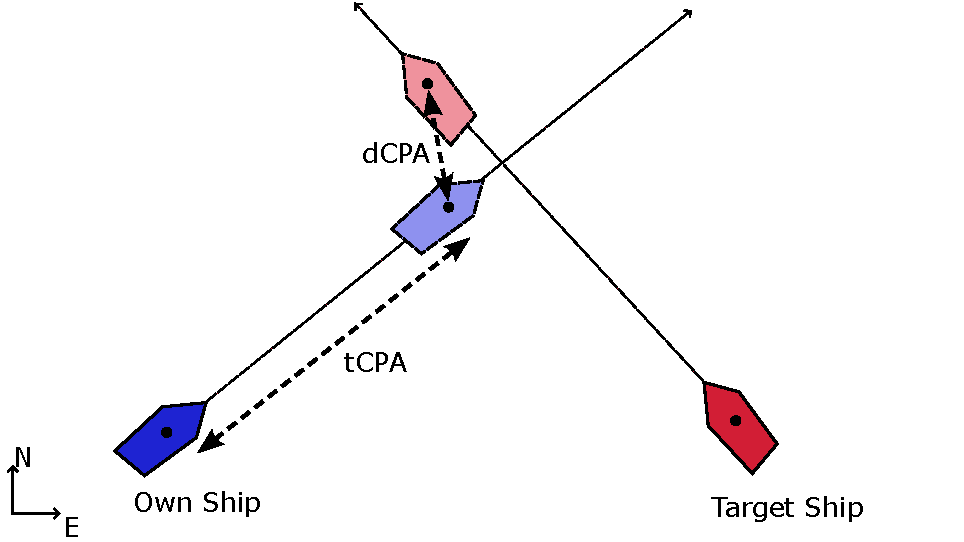
\includegraphics[width=0.8\textwidth]{Images/shipCPA.pdf}
    \caption{Visualizing dCPA and tCPA.}
    \label{FIG: ship CPA}
\end{figure}

These rules are not easily explained to a layperson, and even less easily to a computer algorithm. To formulate the constraints that will
enforce \gls{COLREGs} compliance it is sensible to start by considering rule 7; is there any risk of collision between the \gls{OS}
and any other vessel? A common risk assessment tool is to calculate the \gls{dCPA} and \gls{tCPA} between two vessels as shown by \cite{Kufoalor2018} and Figure \ref{FIG: ship CPA}:
\begin{subequations}    \label{eq:tCPAdCPA}
    \begin{equation}
        t_{AB}^{CPA} = 
        \begin{cases}
          \frac{\textbf{P}_{BA} \cdot \textbf{V}_{A|B}}{||\textbf{V}_{A|B}||^2} & \text{if}\ ||\textbf{V}_{A|B}|| > 0 \\
          0 & \text{otherwise}
        \end{cases}
    \end{equation}
    \begin{equation}
        d_{AB}^{CPA} = ||(\textbf{P}_A + t_{AB}^{CPA} \textbf{V}_A) - (\textbf{P}_B + t_{AB}^{CPA} \textbf{V}_B)||
    \end{equation}
\end{subequations}
where $\textbf{V}_{A|B} = \textbf{V}_A - \textbf{V}_B$ with $\textbf{V}_A$, $\textbf{V}_B$, $\textbf{P}_A$ and $\textbf{P}_B$ being the respective
velocities and positions of two given vessels A and B parameterized in NED. To determine if the \gls{OS} and a given \gls{Ts} should be
considered to be in an active situation, the calculated \gls{dCPA} can be compared to some lower threshold limit. If the \gls{dCPA} is below the set threshold
the next step is to assert which \gls{COLREGs} rule is currently in effect for the \gls{OS}, this is what will be called 'active \gls{COLREGs}
situation' for the rest of this thesis, and asserting which \gls{COLREGs} is currently in effect will be called 'COLREGs classification'.

\begin{figure}[ht!]
    \centering
    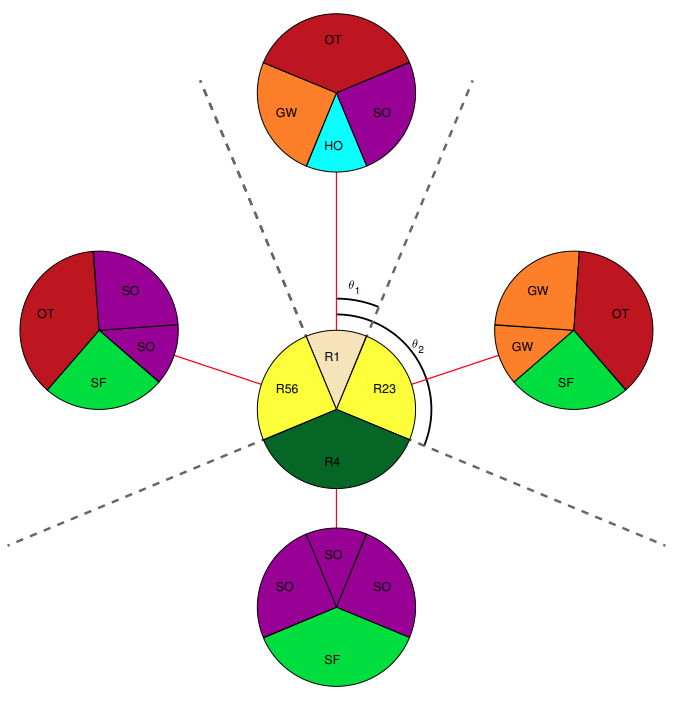
\includegraphics[height=0.6\textheight]{Images/COLREGs_assess.png}
    \caption{COLREGs classifcation; with OS in the center we can place the TS in one of four regions. Similarly the relative bearing from TS to OS can be assigned regions with region 1 pointed directly at the OS and the rest following in a clockwise rotation.
    Courtesy of Emil Thyri.}
    \label{FIG: COLREGs Classification}
\end{figure}
% (Disclaimer: \gls{COLREGs} classification is virtually unchanged from the report delivered as part of the author's fordypningsproject, which is attached
% as an additional file.)
(TODO: denne delen av masteroppgaven er veldig lik fordypningsprosjekt...)
There have been multiple studies on \gls{COLREGs} classification, (\cite{woerner2016multi}) lays out an algorithmic approach based on the
relative bearings between the \gls{OS} and a given \gls{Ts}. In this algorithm numerical values from the \gls{COLREGs} rules are used as the
as the criteria for determining which \gls{COLREGs} sitation the \gls{OS} finds itself in. The algorithm yields the expected results,
but it's a bit opaque and hard to follow. (\cite{tam2010collision}) suggests a similar approach formulated in a more natural language that is easier
and more intuitive to follow. This method first considers the relative bearing from the \gls{Ts} to the \gls{OS}:
\begin{equation}
    \phi = \textrm{atan2}((E_{TS} - E) , (N_{TS} - N)) - \chi
\end{equation}
where $(N_{TS}, E_{TS})$ and $(N, E)$ are the positions of the \gls{Ts} and \gls{OS} respectively, and $\chi$ is the course of the \gls{OS}.
With the \gls{OS} as a centerpiece, 4 sectors can be defined by angles offset from the \gls{OS}'s course, where
the relative bearing $\phi$ deciding which sector the \gls{Ts} is in. Similarly the relative bearing from the \gls{Ts} to the \gls{OS} can be
used to determine \gls{COLREGs} situation. See Figure \ref{FIG: COLREGs Classification} for a visualization.


With \gls{COLREGs} situation classified the last step is to determine the constraints so that the \gls{OS} behaves compliant with the rules.
One method, which was written about in the author's fordypningsproject is to add circular regions as consrtaints tied to the position and heading
of the \gls{Ts} in which the \gls{OS} is in an active situation with. An example of what a singular constraint placed like this would look like
can be seen in Figure \ref{FIG: Dynamic Constraint Example}. To achieve this the trajectory of the \gls{Ts} must be discretized with the same
time step size as the \gls{OS}. At each control interval in the \gls{NLP}, using the known values for the heading 
and position of the \gls{Ts} at that instance $\psi_{TS_{k}}$, $(N_{TS_{k}}, E_{TS_{k}})$, calculate an appropriate constraint origin:
\begin{equation}
    \mathbf{o_{dc}} = \begin{bmatrix}
        N_{TS_{k}} & E_{TS_{k}}
                    \end{bmatrix} + H * \begin{bmatrix}
                                        \cos(\phi_c) \\
                                        sin(\phi_c)
                                        \end{bmatrix}
\end{equation}
where H is the desired distance from the center of the \gls{Ts} to the constraint origin, and $\phi_c$ is the desired relative
bearing from the \gls{Ts} to the constraint origin. The constraints are added to $\textbf{g}(\omega)$ the following way:
\begin{equation} \label{EQ: dynamic constraint in g}
    \textbf{g}(\omega) = \begin{bmatrix}
        \vdots \\
        ||\textbf{X}_k - \mathbf{o_{dc}}||\\
        \vdots
    \end{bmatrix}
\end{equation}
where $\textbf{X}_k$ are the north and east positions in the decision variables $\bm{\omega}$. The square root of the lower bounds value
for $\textbf{g}(\omega)$ denotes the radius of the circle constructed by the consrtraint function, the upper bound value should be infinite.

\begin{figure}[ht]
    \centering
    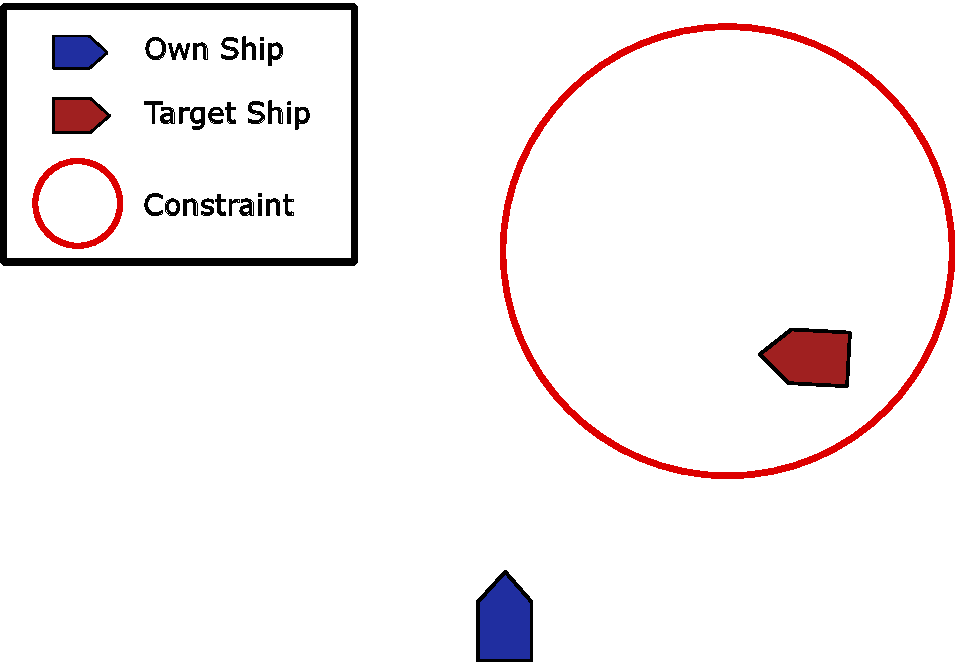
\includegraphics[width=0.8\textwidth]{Images/Constraint_Example.pdf}
    \caption{Example of a single placed constraint based on the position, heading, and COLREGs classification. Depicted would be a suggested
    placement for a Give way situation.}
    \label{FIG: Dynamic Constraint Example}
\end{figure}

% \begin{itemize}
%     \item Segway over to Target ship prediction somehow
%     \item The placement of these dynamic constraints $\mathbf{o_{dc}}$ is vital to the COLREGs compliance of the \gls{OS}.
%     \item 
% \end{itemize}

% However if we are to utilize the advanced prediction we have on other agents a bit more logic must be applied
% to achieve full coverage of our intended path. Presume that our path contains a set of waypoints we intend to pass by, and similarly we know of a set of waypoints another agent intends to
% pass by. To find the true dCPA and tCPA between our own ship and the target vessel we use equations \eqref{eq:tCPAdCPA} as the situation is when each agent passes by one of their
% waypoints(TODO: TRENGER FIGUR FOR Å VISE BEDRE HVA JEG MENER).  Speed is tougher to account for, unless we know better speed should be assumed to remain constant (TODO: dette hører hjemme i background).

% \subsection{'The Complete System'}
% \begin{itemize}
%     \item Vet ikke helt om dette kapittelet er nødvendig, men jeg lurer på om det er en god ide å skrive litt om nøyaktig hvor i ett fult funksjonelt
%     system jeg forventer at min algoritme passer inn. Hva de andre delene jeg ikke kommer til å skrive om har ansvar for, og hva som forventes av systemene
%     rundt mitt eget.
%     \item Hvis systemet mitt var en sort boks, hvilke inputs og outputs ville det hatt.
% \end{itemize}

% \subsection{Simulator Setup}
% \begin{itemize}
%     \item liten forklaring av hvordan simulatoren funker selv om jeg ikke har laget den.
%     \item f.eks agent structs kan bli viktig.
%     \item Forklar at det er en liten forsjel på hvordan own ship agenten og andre agenter oppdateres, fører til en maksimal 'feil' på 1 meter.
% \end{itemize}

\subsection{Target Ship Prediction}
% --------- Genereal thoughts --------------------------
% \begin{itemize}
%     \item Gjenfortelling fra fordypningsprosjekt, da kalt traffic pattern
%     \item Fant en annen artikkel fra Kina som skrev om nogenlunde det samme, \gls{AIS} data -\> prediksjon
%     \item Skiller seg fra fordypningsprosjekt fordi det er egentlig ikke traffic pattern som er den viktige antagelsen,
%     Det er heller viktig at vi antar det finnes en måte å gjette/vite hvor andre båter vil være fremover i tid.
%     \item Andre metoder for target ship prediction kan være f.eks utvidelse av \gls{AIS} som 
%     inkluderer autonav data for de neste 5 minuttene eller noe lignende.
%     \item Disambiguate Simple and Full prediction.
% \end{itemize}
% ---------- /General Thoughts--------------------------- 
% \begin{itemize}
%     \item Naval navigation is an 'active' task, always looking out for obstacles and making sure the way forward is clear.
%     \item There are no lanes, instead proper conduct is dictated by \gls{COLREGs}, the rules are laid out so that different situations
%     have different rules
%     \item Knowing which situation you are in is half the battle, therefor the ability to predict and estiamte how encounters will happen
%     is a powerful tool. Human navigators do this by experience.
%     \item Autonomous vessels could also predict by experience, that would be the machine learning approach. \gls{AIS} can already provide training data.
%     \item But it could be easier than that, what if \gls{AIS} data packets were expanded to send out autonav data for where a vessel intends to traverse.
%     The assumption here is that vessels using autonav will correct their course when spotting a conflict. Vessels not using autonav would still be able to observe
%     the indended path of other vessels and adjust their plans 'manually'.
%     \item Relying on fully predicting the transit of a target vessel is fragile, relying on a few known waypoints would be much more robust.
%     \item In the end the best solution would be if all vessels could fully communicate their intended path either peer to peer or through
%     a centralized system. Solving conflicting paths would be done on a higher level than individual vessel.
%     \item cite \cite{scholler2021trajectory} for AIS prediction.
%     \item cite \cite{zhang2021collision} For mention of massive AIS data.
%     \item cite ais?? har sett noen gjøre det.
%     \item cite \cite{huang2020ship} to refer to current methods for target ship prediction.
% \end{itemize}
% \begin{itemize}
%     \item If it was not done at the end of previous chapter, \cite{cho2018intent} as one research into target ship prediction.
%     \item Also cite \cite{scholler2021trajectory} on AIS prediction, and \cite{zhang2021collision} on the usage of massive AIS data.
%     \item cite \cite{huang2020ship} as an example of how TS prediction is (not) usually done... might not be needed.
%     \item The apparent \gls{COLREGs} compliance of the trajectory planner and collision avoidance algorithm can only be as 
%     good as it's ability to infer intent and predict the trajectories of other \gls{Ts}s. 
%     Infering intent and tracking other \gls{Ts} is an important task for human navigators, and a key part of collision avoidance.
%     % \item Navigation at sea is an active task, for manned vessels there's an expectation of always having an Officer On Watch, a person
%     % who act as a lookout and continously use all available instruments to assess the situation. This is \gls{COLREGs} 5th rule.
%     \item An \gls{ASV} might have the instruments required to achieve full spatial and situational awareness, but it's ability to
%     fully utilize these instruments is often underdeveloped.
%     \item To adress the issue of intent infering, (\cite{cho2018intent}) proposes a method that provides a decision-making procedure
%     for safe navigation by predicting the maneuvering intent of \gls{Ts}s. In their work, a graphical model is constructed to infer intent by
%     combining an intent model with a dynamic model. Each action of the \gls{Ts} influence the ship's assigned maneuvering intent probability,
%     which denotes a probability that the ship is going to be compliant or non-compliant w.r.t \gls{COLREGs}.
%     \item In another study, (\cite{scholler2021trajectory}) attempts to predict the trajectory of \gls{Ts}s via an estimation scheme consisting
%     of a Long Short-term Memory model in a Generative Adverserial Network configuration. The estimation scheme is backed by historical \gls{AIS} data
%     and outputs a probabilistic heat map of the future trajectory of \gls{Ts}s.
%     \item In a similar sense, (\cite{zhang2021collision}) notes in their survey how massive AIS data can be used for global route optimization by
%     creating set waypoints based on the information extracted from massive AIS data.
%     \item This thesis will make no attempts at implementing a prediction method for tracking and infering the intent of \gls{Ts}s. However it will
%     operate under the assumption that the technology for more accurately predicting the trajectories of \gls{Ts}s is coming, and one of the key points
%     of study for this thesis is the question of how improved prediction capacity will affect the behaviour of the proposed trajectory planning algorithm.
%     \item In this thesis, the prediction capabilities afforded to the algorithm will be one of two options.\newline
%     1. 'simple prediction' which is simply assuming that \gls{Ts} will maintain a steady speed and course over ground, 
%     a common method as noted by (\cite{huang2020ship}) in their review. \newline
%     2. 'full prediction' which is some nebulous futuristic interaction and intent aware prediction method that is able to accurately predict the
%     future trajectory of \gls{Ts}.
%     \item Even if the 'full prediction' capabilities are a far off possibility, an intermediate step could be extending the information sent via
%     common AIS transponders, as these are becoming more and more common in smaller vessel, and mandatory in bigger ones. The extended AIS data could
%     include auto-navigation data or other details on the vessels's intended near-future maneuvers, perhaps a list of waypoints and the temporal
%     constraints for reaching them or something similar. Having information is always better than predicting or infering intent, any aiding data that can
%     assist in correcting the predictions made by a computer would massively benefit the development of a 'full prediction' capable algorithm.
% \end{itemize}
The apparent \gls{COLREGs} compliance of the trajectory planner and collision avoidance algorithm can only be as 
good as it's ability to infer intent and predict the trajectories of other \gls{Ts}s. 
Infering intent and tracking other \gls{Ts} is an important task for human navigators, and a key part of collision avoidance.
An \gls{ASV} might have the instruments required to achieve full spatial and situational awareness, but it's ability to
fully utilize these instruments is often underdeveloped.

(TODO: BRIDGE THIS GAP.)\newline
To adress the issue of intent infering, (\cite{cho2018intent}) proposes a method that provides a decision-making procedure
for safe navigation by predicting the maneuvering intent of \gls{Ts}s. In their work, a graphical model is constructed to infer intent by
combining an intent model with a dynamic model. Each action of the \gls{Ts} influence the ship's assigned maneuvering intent probability,
which denotes a probability that the ship is going to be compliant or non-compliant w.r.t \gls{COLREGs}.
In another study, (\cite{scholler2021trajectory}) attempts to predict the trajectory of \gls{Ts}s via an estimation scheme consisting
of a Long Short-term Memory model in a Generative Adverserial Network configuration. The estimation scheme is backed by historical \gls{AIS} data
and outputs a probabilistic heat map of the future trajectory of \gls{Ts}s.

\begin{figure}[ht!]
    \includegraphics[width=0.8\textwidth]{Images/AISLanes.jpg}
    \centering
    \caption{Photo of a typical ENC, here we can see the lines formed by saving AIS positional data over time. Image courtesy of Olex AS.}
    \label{FIG: AIS lanes}
\end{figure}


(TODO: BRIDGE THIS GAP.)\newline
In a similar sense, (\cite{zhang2021collision}) notes in their survey how massive AIS data can be used for global route optimization by
creating set waypoints based on the information extracted from massive AIS data.
This AIS data can easily be compiled by storing the positional data of AIS transpoders over a period of time, as see in Figure \ref{FIG: AIS lanes}, which
is the result of saving data for about three days.


This thesis will make no attempts at implementing a prediction method for tracking and infering the intent of \gls{Ts}s. However it will
operate under the assumption that the technology for more accurately predicting the trajectories of \gls{Ts}s is coming, and one of the key points
of study for this thesis is the question of how improved prediction capacity will affect the behaviour of the proposed trajectory planning algorithm.
In this thesis, the prediction capabilities afforded to the algorithm will be one of two options.\newline
1. 'simple prediction' which is simply assuming that \gls{Ts} will maintain a steady speed and course over ground, 
a common method as noted by (\cite{huang2020ship}) in their review. \newline
2. 'full prediction' which is some nebulous futuristic interaction and intent aware prediction method that is able to accurately predict the
future trajectory of \gls{Ts}.

(TODO: siste avsnitt passer kanskje bedre i discussion.)\newline
Even if the 'full prediction' capabilities are a far off possibility, an intermediate step could be extending the information sent via
common AIS tde auto-navigation data or other details on the vessels's intended near-future maneuvers, perhaps a list of waypoints and the temporal
constraints for reaching them or something similar. Having information is always better than predicting or infering intent, any aiding data that can
assist in correctiransponders, as these are becoming more and more common in smaller vessel, and mandatory in bigger ones. The extended AIS data could
inclung the predictions made by a computer would massively benefit the development of a 'full prediction' capable algorithm.



\newpage